\documentclass[12pt]{article}
%%% DOCUMENT FORMATTING %%%
\usepackage[margin=1in]{geometry}
\usepackage{enumitem}
\setlength{\parindent}{0pt}
\newcommand{\disp}{\displaystyle}

%%% HEADER %%%
\usepackage{fancyhdr}
\pagestyle{fancy}
\fancyhf{}
\lhead{MATH 1060}
\rhead{Vagnozzi}
\cfoot{\thepage}

%%% MATH NOTATION & SYMBOLS %%%
\usepackage{amssymb}
\usepackage{amsmath}
\newcommand{\R}{\mathbb{R}}
\newcommand{\N}{\mathbb{N}}
\newcommand{\Z}{\mathbb{Z}}
\newcommand{\lp}{\left(}
\newcommand{\rp}{\right)}
\newcommand{\ls}{\left[}
\newcommand{\rs}{\right]}
\newcommand{\lb}{\left\{}
\newcommand{\rb}{\right\}}
\newcommand{\arccot}{\text{arccot}}
\newcommand{\arccsc}{\text{arccsc}}
\newcommand{\arcsec}{\text{arcsec}} 

%%% TABLES %%%
\usepackage{colortbl}

%%% GRAPHS %%%
\usepackage{tikz}
\usepackage{pgfplots}
\pgfplotsset{compat=1.15}
\usepgfplotslibrary{fillbetween}
\usetikzlibrary{angles,quotes}

%%% ENVIRONMENTS %%%
\newcommand{\Example}{\paragraph{\Writinghand \hspace{0.1mm} Example.}}
\newcommand{\ExampleCont}{\paragraph{\Writinghand \hspace{0.1mm} Example (continued).}}
\newcommand{\boxenv}[2]{
	\fbox{
	\begin{minipage}{0.97\textwidth}
	\vspace{2mm}	
	\paragraph{#1} #2
	\vspace{2mm}
	\end{minipage}
	}}

%%% FUN THINGS %%%
\newcommand*\tc[1]{\tikz[baseline=(char.base)]{
            \node[shape=circle,draw,inner sep=2pt] (char) {#1};}}
\usepackage{marvosym}

%%% MISC %%%
\usepackage{hyperref}


\setcounter{page}{137}

\begin{document}
\section*{4.6: Linear Approximation and Differentials}

\boxenv{Learning Objectives.}{Upon successful completion of Section 4.6, you will be able to\dots
		
	\begin{itemize}[leftmargin=6mm]
		\item Answer conceptual questions involving linear approximation and differentials.
		\item Find a linear approximation function.
		\item Write a linear approximation function, and estimate the value of a function and \\ evaluate the error.
		\item Choose a value ot minimize error and use it to write a linear approximation of a quantity.
		\item Graph a function and its linear approximation to identify overestimates and \\ underestimates.
		\item Solve applications involving linear approximations.
		\item Given a function, write a differential expression expressing the change in the dependent variable as a function of a change in the independent variable.
	\end{itemize}
	\vspace{-4mm}
}

\vspace{5mm}

\subsection*{Linear Approximation}

Differentiable functions are said to be \textbf{locally linear}. In other words, if we ``zoom in'' really closely, the function may appear to be linear. Recall the definition of a linear function.

\vspace{5mm}

\boxenv{Definition.}{A \textbf{linear function} has the form $f(x)=mx+b$, where $m$ is the slope and $(0,b)$ is the $y$-intercept. The domain and range is $\R$.}

\vspace{5mm}

\paragraph{Motivation.} Suppose $f$ is differentiable at $x=c$ and let $L$ represent the tangent line centered at $x=c$. If $x$ is ``near'' $c$, then

$$\big| f(x)-L(x)\big| \approx 0 \, \Longleftrightarrow \, f(x)\approx L(x).$$

\vspace{3mm}

In other words, the linear function defined by the tangent line at $x=c$ may serve as a ``good'' approximation to the function $f$ so long as we don't stray too far from the center. 

\vspace{3mm}

Linear approximation is especially useful in situations when $f$ involves non-algebraic operations that are difficult (or impossible) to evaluate by hand.

\begin{center}
            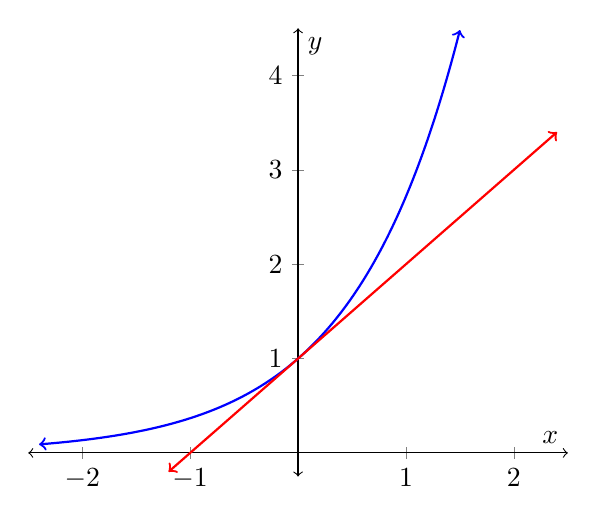
\begin{tikzpicture}
                \begin{axis}[
                	axis x line=center,
                	xmax=2.5, xmin=-2.5,
                	axis y line=center,
                	ymax=4.5, ymin=-0.25,
                	xlabel=$x$,ylabel=$y$,
                	axis line style=<->
                    ]
                    \addplot[name path=f,smooth,domain=-2.4:1.5,color=blue,samples=100,<->,thick] {e^x};
                    \addplot[name path=f,smooth,domain=-1.2:2.4,color=red,samples=100,<->,thick] {1+x};
                \end{axis}
            \end{tikzpicture}
		$$ f(x) \approx L(x) \text{ for } x \text{ ``near'' the center of the tangent line}$$
        \end{center}
        
        \vspace{5mm}
        
\boxenv{Definition.}{The \textbf{linearization}, $L$, of $f$ at $x=c$ is defined by
$$y-f(c)=f'(c)(x-c) \,\Longrightarrow\, \fbox{$L(x)=f(c)+f'(c)(x-c)$}$$
so long as $f$ is continuous and differentiable at $x=c$. 
}

\vspace{5mm}

This is sometimes referred to as the \textit{degree-1 Taylor polynomial}.

\vspace{3mm}

For purposes of approximation, the linearization takes the place of the function. For example, to estimate $f(4.2)$, we can find $L(4.2)$ instead.

\vspace{3mm}

\Example Write the linearization of $f(x)=e^x$ at $x=0$. Use this to find a linear approximation for $\sqrt[5]{e}$.

\newpage

\ExampleCont Suppose we'd now like to approximate $e^2$ using the previous linearization. Explain why the approximation will be less accurate.

\vspace{35mm}

\Example Find a linear approximation for $f(2.1)$ if $f(x)=12-x^2$.

\vspace{50mm}

\Example Find a linear approximation for $\sqrt[3]{25}$.

\vspace{50mm}

\Example Find a linear approximation for $\sqrt{500}$.

\newpage

\paragraph{Error and Concavity.} The \textit{concavity} of a function can help explain the \textbf{accuracy} of a linear approximation.
\begin{itemize}
\item If $f''$ is ``small'' at the center of the linearization, the curvature is only slight, so the tangent line ``hugs'' the graph relatively tightly. This leads to a \textit{smaller} error in the approximation.
\item If $f''$ is ``large'' at the center of the linearization, the curvature is very pronounced, so the tangent line does not ``hug'' the graph for very long, and the error in the approximation will be \textit{larger}.
\end{itemize}

Hence, a linear approximation works best when $f''$ is relatively small in magnitude.

\vspace{5mm} 

Once we have an approximation, we are able to say whether the approximation is an \textit{underestimate} or \textit{overestimate} of the true function value.

\vspace{5mm}

\boxenv{Theorem.}{Suppose $f$ is twice-differentiable at $x=c$. 
\begin{itemize}
\item If $f''(c)<0$, then $L(c)$ is an overestimate of $f(c)$.
\item If $f''(c)>0$, then $L(c)$ is an underestimate of $f(c)$.
\end{itemize}

\vspace{-3mm}
}


\vspace{3mm}

\Example Find a linear approximation for $\ln(2)$ and determine if the approximation is an underestimate or overestimate.

\newpage

\subsection*{Differentials}

While linear approximation allows us to estimate the $y$-value itself, \textbf{differentials} allow us to estimate the \textit{change} in the $y$-value, $\Delta y$, for a small change in the $x$-value, $\Delta x$. 

\vspace{60mm}

Using a linear approximation, we could say that $\Delta y\approx \Delta L$.

\vspace{60mm}

If $x=c$ changes to $x=c+\Delta x$, then \underline{\hspace{35mm}}.

\vspace{5mm}

We introduce the \textbf{infinitesimals} $dy$ and $dx$ to replace $\Delta L$ and $\Delta x$.

\vspace{5mm}

\boxenv{Definition.}{The difference $f(x+dx)-f(x)$ is called the \textbf{increment} or \textbf{change} in $f$ and is denoted by $\Delta y$.}

\vspace{5mm}

\boxenv{Definition.}{If $f$ is differentiable, the product $f'(x)dx$ is called the \textbf{differential} and is denoted by $dy$, i.e.\ $dy=f'(x)dx$.}

\newpage

\Example Let $y=e^x$. Suppose that $x$ increases from $x=0$ to $x=\disp\frac{1}{4}$. By about how much will the $y$-value change?

\vspace{60mm}

\Example Let $y=\arctan(x)$. Suppose that $x$ decreases from $x=1$ to $x=\disp\frac{9}{10}$. By about how much will the $y$-value change?

\vspace{60mm}

\Example Let $y=\sin(x)$. Suppose that $x$ increases from $x=\disp\frac{\pi}{3}$ to $x=\disp\frac{\pi}{3}+0.05$. By about how much will the $y$-value change?

\newpage

\Example Use a differential to approximate $\sqrt{146}$.

\vspace{60mm}

\Example Suppose the radius of a circle decreases from $r=5$ cm to $r=4.25$ cm. By about how much will the area of the circle change?

\vspace{60mm}

\paragraph{Accuracy.} Much like in linearization, the accuracy of an estimate using differentials relies on ``staying close'' to the center value of $x=c$. $dx$ should be ``small'' in order for the approximation to be useful.

\vspace{5mm}

For example, consider the following differentials for $y=e^x$ centered at $c=0$. The values of $dy$ are fairly accurate estimates of $\Delta y$ when $dx$ is small, but as $dx$ grows larger, the differential is less accurate.

\begin{center}
\begin{tabular}{|
>{\columncolor[HTML]{EFEFEF}}c |c|c|}
\hline
$dx$                                                 & $dy$                        & $\Delta y$     \\ \hline
$0.01$                                               & $0.01$                      & $0.0101$                      \\ \hline
$0.10$                                               & $0.10$                      & $0.1052$                      \\ \hline
$0.50$                                               & $0.50$                      & $0.6487$                      \\ \hline
$1.00$                                               & $1.00$                      & $1.7183$                      \\ \hline
\multicolumn{1}{|l|}{\cellcolor[HTML]{EFEFEF}$2.00$} & \multicolumn{1}{l|}{$2.00$} & \multicolumn{1}{l|}{$6.3891$} \\ \hline
\end{tabular}
\end{center}

In fact, $\disp\lim_{dx\to\pm\infty}\big|\Delta y-dy\big|=\infty$.


\end{document}